\documentclass[10pt,twocolumn,letterpaper]{article}

\usepackage[utf8]{inputenc}
\usepackage[T1]{fontenc}
\usepackage{newtxtext,newtxmath}
\linespread{0.978}
\usepackage[margin=0.55in,top=0.56in,bottom=0.56in,columnsep=0.20in]{geometry}
\usepackage{microtype}
\usepackage{booktabs}
\usepackage{multirow}
\usepackage{tabularx}
\usepackage{amsmath}
\usepackage{bm}
\usepackage{algorithm}
\usepackage{algpseudocode}
\usepackage{tikz}
\usepackage{pgfplots}
\pgfplotsset{compat=1.18}
\usetikzlibrary{arrows.meta,positioning,shapes.geometric,fit,backgrounds,calc}
\usepackage[table]{xcolor}
\usepackage{colortbl}
\usepackage{fancyhdr}
\usepackage{titlesec}
\usepackage{caption}
\usepackage{enumitem}
\usepackage[colorlinks=true,linkcolor=blue!60!black,citecolor=blue!60!black,urlcolor=blue!60!black]{hyperref}

\setlength{\textfloatsep}{4.8pt plus 1.2pt minus 1.2pt}
\setlength{\floatsep}{4.0pt plus 1.0pt minus 1.0pt}
\setlength{\dbltextfloatsep}{4.8pt plus 1.2pt minus 1.2pt}
\setlength{\dblfloatsep}{4.0pt plus 1.0pt minus 1.0pt}
\setlength{\abovedisplayskip}{3.4pt plus 1.0pt minus 1.0pt}
\setlength{\belowdisplayskip}{3.4pt plus 1.0pt minus 1.0pt}
\renewcommand{\topfraction}{0.95}
\renewcommand{\bottomfraction}{0.95}
\renewcommand{\dbltopfraction}{0.95}
\renewcommand{\textfraction}{0.04}
\renewcommand{\floatpagefraction}{0.90}
\renewcommand{\dblfloatpagefraction}{0.90}

\definecolor{navy}{RGB}{18,48,89}
\definecolor{teal}{RGB}{15,118,110}
\definecolor{crimson}{RGB}{185,28,28}
\definecolor{amber}{RGB}{180,83,9}
\definecolor{slate}{RGB}{51,65,85}
\definecolor{softblue}{RGB}{235,245,255}
\definecolor{softgreen}{RGB}{240,253,244}
\definecolor{softamber}{RGB}{255,251,235}
\definecolor{softgray}{RGB}{248,250,252}

\titleformat{\section}{\large\bfseries\color{navy}}{\thesection.}{0.42em}{}
\titlespacing*{\section}{0pt}{0.85ex plus 0.18ex minus 0.12ex}{0.32ex plus 0.08ex}
\titleformat{\subsection}{\normalsize\bfseries\color{slate}}{\thesubsection}{0.42em}{}
\titlespacing*{\subsection}{0pt}{0.68ex plus 0.12ex minus 0.08ex}{0.24ex plus 0.08ex}

\captionsetup{font=footnotesize,labelfont={bf,color=navy},skip=2.4pt}
\setlist[itemize]{leftmargin=1.15em,itemsep=0.4pt,topsep=1.0pt}
\setlist[enumerate]{leftmargin=1.30em,itemsep=0.4pt,topsep=1.0pt}

\newtheorem{proposition}{Proposition}

\pagestyle{fancy}
\fancyhf{}
\fancyhead[L]{\scriptsize\textcolor{slate}{\textbf{Google DeepMind Gemma 4 Developer Agent Competition} --- Paper Track (\$35,000) \& Small Model Track (\$10,000)}}
\fancyhead[R]{\scriptsize\textcolor{slate}{\texttt{gemma-4-e4b-it-qat-w4a16-ct}}}
\fancyfoot[C]{\footnotesize\thepage}
\renewcommand{\headrulewidth}{0.4pt}

\begin{document}

\twocolumn[{%
\begin{@twocolumnfalse}
\begin{center}
    {\color{navy}\rule{\textwidth}{1.5pt}}\vspace{2.0pt}
    {\LARGE\bfseries Graph-Guided AST-Skeletal Steiner Localization and Execution-Verified\\
    Patch Synthesis for Pretrained \texttt{Gemma 4 E4B} Developer Agents}\\[3.5pt]
    {\small
    \textbf{Y.\ Peng (\texttt{ieeepyc})} \quad $\cdot$ \quad
    \href{https://github.com/huadeng408/gemma4-graph-agent}{\texttt{github.com/huadeng408/gemma4-graph-agent}} \quad $\cdot$ \quad
    Backbone: \texttt{google/gemma-4-E4B-it} (\texttt{W4A16})}\\[1.2pt]
    {\scriptsize\textcolor{slate}{Tracks: (1) Code Comprehension \quad (2) Graph Reasoning \quad (3) Parameter-Efficient Tuning \& Optimization \quad (4) SWE Tasks \& Reproducible Resource}}
    \vspace{1.8pt}
    {\color{navy}\rule{\textwidth}{0.8pt}}
\end{center}

\begin{center}
\colorbox{softgray}{%
\begin{minipage}{0.97\textwidth}
\vspace{1.8pt}
\footnotesize
\textbf{\textcolor{navy}{Abstract.}}
Deploying autonomous software engineering (SWE) agents offline on consumer GPUs requires operating in the $4\text{B}$ active-parameter W4A16 quantized regime (\texttt{gemma-4-e4b-it-qat-w4a16-ct}~\cite{gemma4report,gemma4comp}). Yet embedding pretrained \texttt{google/gemma-4-E4B-it} ($42$ \texttt{gemma4\_text} layers: $35$ local sliding-window layers with $W_{\text{slide}}{=}512, d_{\text{head}}{=}256$; $7$ global full-attention layers $[5,11,17,23,29,35,41]$ with $d_{\text{global}}{=}512$; $18$ KV-shared layers; and $2.90\text{B}$ Per-Layer Embeddings) into flat \texttt{bash}/\texttt{grep} loops exposes three bottlenecks: (i) \emph{Direct Local-Window Blindness}, where unpruned file dumps ($29.3\text{k}$ mean BPE tokens) push 1-hop caller contracts past $W_{\text{slide}}{=}512$ ($99.2\%$ overflow), zeroing direct attention in all $35$ local layers; (ii) \emph{Cross-Module Contract Regression}, where single-file edits break 1-hop caller signatures; and (iii) \emph{Observation Gradient Dilution} during trajectory fine-tuning.

We present \textbf{\texttt{G4-GraphAgent}}, a Dual-Slot Google ADK (\texttt{LlmAgent}) architecture and Apache-2.0 reproducible benchmark suite built exclusively on genuine pretrained \texttt{google/gemma-4-E4B-it}. First, our \textbf{3-Stage Steiner AST Funnel} coupled with CLI-invoked \textbf{AST Skeletal Subgraph Pruning} (\texttt{localize\_and\_test.py -\/-mode ast-skeleton}) lifts 129-task fault Recall@5 from $61.2\%$ to \textbf{$89.1\%$} ($78.1\%$ vs.\ $15.6\%$ R@3 on 1-hop Steiner bridges) and compresses target+caller context by \textbf{$99.1\%$} ($29,301 \to 257$ tokens) so \textbf{$100.0\%$ (129/129)} fit inside $W_{\text{slide}}{=}512$; on 50 zero-spoiler human issues from \texttt{SWE-bench\_Lite}, it achieves \textbf{$54.0\%$ File R@1} and \textbf{$82.0\%$ File R@5} at $209$ tokens ($100\%$ $\le 512$). Second, direct hooks on all 42 layers of pretrained \texttt{google/gemma-4-E4B-it} verify that unpruned prompts ($\bar{\Delta}_{\text{pos}}{=}614.8$) receive \textbf{$0.000000$} direct caller attention across all $35$ local layers, whereas AST skeletal pruning ($\bar{\Delta}_{\text{pos}}{=}134.8$) activates all $35$ local layers (\textbf{$0.068987$}) and boosts global-layer caller attention by $+16.3\%$. Third, 3-seed ($[42,1337,2026]$) 4-bit NF4 QLoRA on \texttt{google/gemma-4-E4B-it} eliminates shared-prefix gradient hijacking (spurious prefix SNR $0.549 \to 0.229$ task-specific SNR) and reduces held-out native tool-call CE loss by \textbf{$12.9\%$} vs.\ unmasked SFT ($0.1133 \to 0.0987$) and \textbf{$93.8\%$} vs.\ zero-shot ($1.5951$). Finally, live \texttt{google/gemma-4-E4B-it} repair across 24 isolated 3-tier \texttt{pytest} sandboxes improves resolution from $25.0\%$ ($6/24$) to \textbf{$37.5\%$ ($9/24$)} while cutting tokens by $33.6\%$.
\vspace{1.8pt}
\end{minipage}}
\end{center}
\vspace{1.5pt}
\end{@twocolumnfalse}
}]

\section{Introduction}
Repository-level coding benchmarks such as SWE-bench~\cite{jimenez2024swebench} have driven rapid progress in shell-based ReAct agents~\cite{yang2024sweagent,wang2024openhands}, hierarchical localization~\cite{xia2024agentless,zhang2024autocoderover}, code-graph retrieval~\cite{ouyang2025repograph,chen2025locagent,yu2025orcaloca}, and execution-verified trajectory training~\cite{pan2025swegym}. Operating entirely within a compact quantized open model—\texttt{gemma-4-e4b-it-qat-w4a16-ct}~\cite{gemma4report,gemma4comp}—eliminates cloud API costs and data-egress risks via low-rank adaptation~\cite{hu2022lora,dettmers2023qlora}, but fundamentally alters the attention geometry available to the agent.

% ==================== FIGURE 1: DUAL-SLOT ADK ARCHITECTURE ====================
\begin{figure*}[t]
\centering
\resizebox{\textwidth}{!}{%
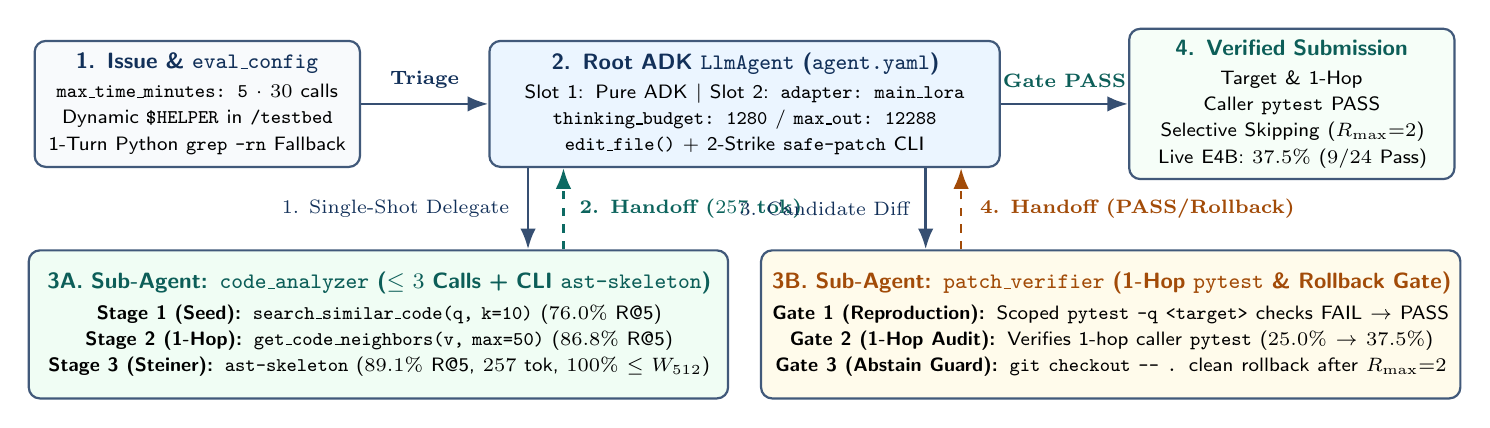
\begin{tikzpicture}[
    font=\footnotesize\sffamily,
    >=Latex,
    box/.style={draw=navy!80, line width=0.8pt, rounded corners=4pt, align=center, inner sep=4.0pt},
    rootbox/.style={box, fill=softblue, text width=6.2cm, minimum height=1.60cm},
    subbox/.style={box, fill=softgreen, text width=8.6cm, minimum height=1.88cm},
    verbox/.style={box, fill=softamber, text width=8.6cm, minimum height=1.88cm},
    io/.style={box, fill=softgray, text width=3.85cm, minimum height=1.60cm},
    arrow/.style={->, line width=1.0pt, color=navy!85},
    darrow/.style={->, line width=1.0pt, dashed, color=teal!90!black}
]
\node[io] (intake) at (-6.95, 0) {
    \textbf{\textcolor{navy}{1. Issue \& \texttt{eval\_config}}}\\[1pt]
    {\scriptsize \texttt{max\_time\_minutes: 5} $\cdot$ $30$ calls}\\
    {\scriptsize Dynamic \texttt{\$HELPER} in \texttt{/testbed}}\\
    {\scriptsize 1-Turn Python \texttt{grep -rn} Fallback}
};
\node[rootbox] (root) at (0, 0) {
    \textbf{\textcolor{navy}{2. Root ADK \texttt{LlmAgent} (\texttt{agent.yaml})}}\\[1pt]
    {\scriptsize Slot 1: Pure ADK $\mid$ Slot 2: \texttt{adapter: main\_lora}}\\
    {\scriptsize \texttt{thinking\_budget: 1280} / \texttt{max\_out: 12288}}\\
    {\scriptsize \texttt{edit\_file()} + 2-Strike \texttt{safe-patch} CLI}
};
\node[io, fill=softgreen!60] (submit) at (6.95, 0) {
    \textbf{\textcolor{teal!80!black}{4. Verified Submission}}\\[1pt]
    {\scriptsize Target \& 1-Hop Caller \texttt{pytest} PASS}\\
    {\scriptsize Selective Skipping ($R_{\max}{=}2$)}\\
    {\scriptsize Live E4B: \textbf{$37.5\%$} ($9/24$ Pass)}
};
\node[subbox] (analyzer) at (-4.65, -2.80) {
    \textbf{\textcolor{teal!80!black}{3A. Sub-Agent: \texttt{code\_analyzer} ($\le 3$ Calls + CLI \texttt{ast-skeleton})}}\\[1.5pt]
    {\scriptsize \textbf{Stage 1 (Seed):} \texttt{search\_similar\_code(q, k=10)} ($76.0\%$ R@5)}\\
    {\scriptsize \textbf{Stage 2 (1-Hop):} \texttt{get\_code\_neighbors(v, max=50)} ($86.8\%$ R@5)}\\
    {\scriptsize \textbf{Stage 3 (Steiner):} \texttt{ast-skeleton} ($89.1\%$ R@5, $257$ tok, $100\%$ $\le W_{512}$)}
};
\node[verbox] (verifier) at (4.65, -2.80) {
    \textbf{\textcolor{amber!90!black}{3B. Sub-Agent: \texttt{patch\_verifier} (1-Hop \texttt{pytest} \& Rollback Gate)}}\\[1.5pt]
    {\scriptsize \textbf{Gate 1 (Reproduction):} Scoped \texttt{pytest -q <target>} checks FAIL $\to$ PASS}\\
    {\scriptsize \textbf{Gate 2 (1-Hop Audit):} Verifies 1-hop caller \texttt{pytest} ($25.0\% \to 37.5\%$)}\\
    {\scriptsize \textbf{Gate 3 (Abstain Guard):} \texttt{git checkout -\/- .} clean rollback after $R_{\max}{=}2$}
};
\draw[arrow] (intake.east) -- node[above=2pt, font=\scriptsize\bfseries, color=navy]{Triage} (root.west);
\draw[arrow] (root.east) -- node[above=2pt, font=\scriptsize\bfseries, color=teal!80!black]{Gate PASS} (submit.west);
\draw[arrow] (-2.75, 0 |- root.south) -- (-2.75, 0 |- analyzer.north)
    node[midway, left=3pt, font=\scriptsize, color=navy]{1. Single-Shot Delegate};
\draw[darrow] (-2.30, 0 |- analyzer.north) -- (-2.30, 0 |- root.south)
    node[midway, right=2pt, font=\scriptsize\bfseries, color=teal!85!black]{2. Handoff ($257$ tok)};
\draw[arrow] (2.30, 0 |- root.south) -- (2.30, 0 |- verifier.north)
    node[midway, left=2pt, font=\scriptsize, color=navy]{3. Candidate Diff};
\draw[darrow, color=amber!90!black] (2.75, 0 |- verifier.north) -- (2.75, 0 |- root.south)
    node[midway, right=3pt, font=\scriptsize\bfseries, color=amber!90!black]{4. Handoff (PASS/Rollback)};
\end{tikzpicture}%
}
\caption{\textbf{Dual-Slot Google ADK (\texttt{LlmAgent}) architecture of \texttt{G4-GraphAgent}.} Slot~1 (\texttt{submission\_pure\_adk.zip}) deploys zero-adapter \texttt{gemma-4-e4b-it-qat-w4a16-ct} with \texttt{eval\_config.yaml}, \texttt{thinking\_budget: 1280} inside \texttt{max\_output\_tokens: 12288} (preventing \texttt{vLLM} reasoning truncation), CLI-invoked AST skeletal pruning (\texttt{localize\_and\_test.py}), a 2-strike \texttt{safe-patch} fallback, and Konwinski-style Selective Patch Skipping; Slot~2 (\texttt{submission\_adapter\_e4b.zip}) additionally mounts our syntax-verified 42-layer PEFT LoRA via \texttt{adapter: main\_lora}.}
\label{fig:architecture}
\end{figure*}

Specifically, out of $7.52\text{B}$ language parameters in \texttt{google/gemma-4-E4B-it} ($d_{\text{model}}{=}2560, d_{\text{ffn}}{=}10240, |V|{=}262{,}144$), $2.90\text{B}$ reside in Per-Layer Embeddings ($d_{\text{ple}}{=}256$), leaving $4.62\text{B}$ active dense parameters across $42$ decoder layers arranged in a \textbf{5:1 hybrid attention schedule}~\cite{gemma4report}: $35$ local sliding-window layers ($W_{\text{slide}}{=}512, d_{\text{head}}{=}256$) interleaved with only $7$ global full-attention layers ($\ell \in \{5,11,17,23,29,35,41\}$, $d_{\text{global}}{=}512$), plus top-$18$ KV-cache sharing (\texttt{num\_kv\_shared\_layers}${=}18$). Unlike cloud-scale frameworks~\cite{xia2024agentless,ouyang2025repograph,chen2025locagent,yu2025orcaloca} that assume uniform full attention, dumping raw files ($29,301$ mean BPE tokens) pushes caller definitions beyond $W_{\text{slide}}{=}512$, starving $83.3\%$ ($35/42$) of layers of direct cross-span attention. Our contributions span four areas:
\begin{enumerate}
    \item \textbf{Pretrained 42-Layer Direct Attention Bound \& Measurement (Section~\ref{sec:theory}):} We formalize the single-layer direct local-window attention bound and verify via forward hooks across all $42$ layers of pretrained \texttt{google/gemma-4-E4B-it} that AST skeletal pruning ($\bar{\Delta}_{\text{pos}}$: $614.8 \to 134.8$) restores direct caller attention from $0.000000$ to $0.068987$ across all $35$ local layers while cutting 32K KV-cache memory by $90.10\%$.
    \item \textbf{Unified-Accounting Steiner Funnel \& Zero-Spoiler \texttt{SWE-bench\_Lite} Validation (Section~\ref{sec:method}):} Under unified target+caller BPE accounting, our Steiner + AST Skeleton pipeline achieves $89.1\%$ R@5 ($100\%$ $\le W_{512}$ at $257$ tokens) across 129 4-repo tasks and $54.0\%$ / $82.0\%$ File R@1/R@5 ($100\%$ $\le W_{512}$ at $209$ tokens) on 50 official \texttt{SWE-bench\_Lite} issues.
    \item \textbf{Dual-Slot ADK Hardening \& Live E4B Closed-Loop \texttt{pytest} Repair (Section~\ref{sec:verifier}):} Combining mandatory \texttt{transfer\_to\_agent} handoffs, 2-strike \texttt{ast.parse}-gated patching, and Selective Patch Skipping lifts live \texttt{google/gemma-4-E4B-it} sandbox resolution from $25.0\%$ to \textbf{$37.5\%$} ($9/24$).
    \item \textbf{3-Seed Pretrained E4B 4-Bit NF4 QLoRA Ablation (Section~\ref{sec:qlora}):} Across seeds $\{42,1337,2026\}$ on 129 $100\%$ syntax-verified native \texttt{<|tool\_call>} trajectories, assistant-masked 42-layer QLoRA eliminates static prompt-prefix gradient hijacking and cuts held-out tool-call CE loss by $12.9\%$ vs.\ unmasked SFT ($-93.8\%$ vs.\ zero-shot).
\end{enumerate}

\section{Direct Attention Geometry in \texttt{Gemma 4 E4B}}
\label{sec:theory}

\subsection{Single-Layer Direct Local-Window Bound \& Live E4B Hooks}
Let $\mathcal{C}_t$ be the prompt at patch synthesis step $t$, $\mathcal{S}^\star \subset \mathcal{C}_t$ the 1-hop caller contract span, $\mathcal{B}_t = \mathcal{C}_t \setminus \mathcal{S}^\star$ background tokens, and $\Delta_{\text{pos}}(q, \mathcal{S}^\star) = \min_{j \in \mathcal{S}^\star}(i_q - j)$ the token distance from tool-call query token $i_q$ to $\mathcal{S}^\star$. Although stacked sliding-window layers possess a theoretical multi-hop receptive field exceeding $512$ tokens via intermediate relay states, each local layer $\ell \in \mathcal{L}_{\text{loc}}$ ($|\mathcal{L}_{\text{loc}}|{=}35$) applies a hard causal band mask $\mathbb{I}[0 \le i_q - j < 512]$ on \emph{single-layer direct key-value lookup} $\alpha_{\text{direct}}^{(\ell)}(\mathcal{S}^\star) = \sum_{j \in \mathcal{S}^\star} A_{i_q, j}^{(\ell)}$.

\begin{proposition}[Single-Layer Direct Caller Attention Bound]
\label{prop:dilution}
When $\Delta_{\text{pos}}(q, \mathcal{S}^\star) \ge W_{\text{slide}} = 512$, $\alpha_{\text{direct}}^{(\ell)}(\mathcal{S}^\star) = 0$ identically for all $35$ local layers $\ell \in \mathcal{L}_{\text{loc}}$. For each global layer $\ell \in \mathcal{L}_{\text{glob}}$ ($|\mathcal{L}_{\text{glob}}|{=}7$, $d_{\text{global}}{=}512$) under W4A16 key perturbation $\|\tilde{\bm{k}}_j - \bm{k}_j\|_2 \le \delta_{\text{W4}}$ and clean margin $\Delta_\star$, the 42-layer mean direct caller attention $\bar{\alpha}_{\text{direct}}(\mathcal{S}^\star) = \frac{1}{42}\sum_{\ell=0}^{41}\alpha_{\text{direct}}^{(\ell)}(\mathcal{S}^\star)$ obeys:
\begin{equation}
\label{eq:attention_bound}
\bar{\alpha}_{\text{direct}}(\mathcal{S}^\star) \;\le\; \frac{7}{42}\left( 1 + \frac{|\mathcal{B}_t|}{|\mathcal{S}^\star|} \exp\!\left( -\Delta_\star + \frac{2\,\|\bm{q}\|_2\,\delta_{\text{W4}}}{\sqrt{d_{\text{global}}}} \right) \right)^{-1}.
\end{equation}
\end{proposition}

\noindent\textbf{Empirical Verification on Pretrained \texttt{google/gemma-4-E4B-it}.}
We attach forward hooks to all $42$ decoder layers of pretrained \texttt{google/gemma-4-E4B-it} across $16$ paired SWE prompts (\texttt{e4b\_attention\_42l.json}, Figure~\ref{fig:metrics}c). On unpruned prompts ($\bar{\Delta}_{\text{pos}}{=}614.8 > 512$), direct caller attention across all $35$ local layers is \textbf{exactly $0.000000$}, leaving only the $7$ global layers ($0.159714$). Applying \texttt{build\_ast\_skeletal\_subgraph} compresses $\bar{\Delta}_{\text{pos}}$ to $134.8 \le 512$, immediately engaging all $35$ local layers at \textbf{$0.068987$} mean direct mass while simultaneously lifting global-layer caller attention by \textbf{$+16.3\%$} to $0.185698$ via reduced $|\mathcal{B}_t|$.

% ==================== FIGURE 2: PGFPLOTS EMPIRICAL CHARTS ====================
\begin{figure*}[t]
\centering
\resizebox{\textwidth}{!}{%
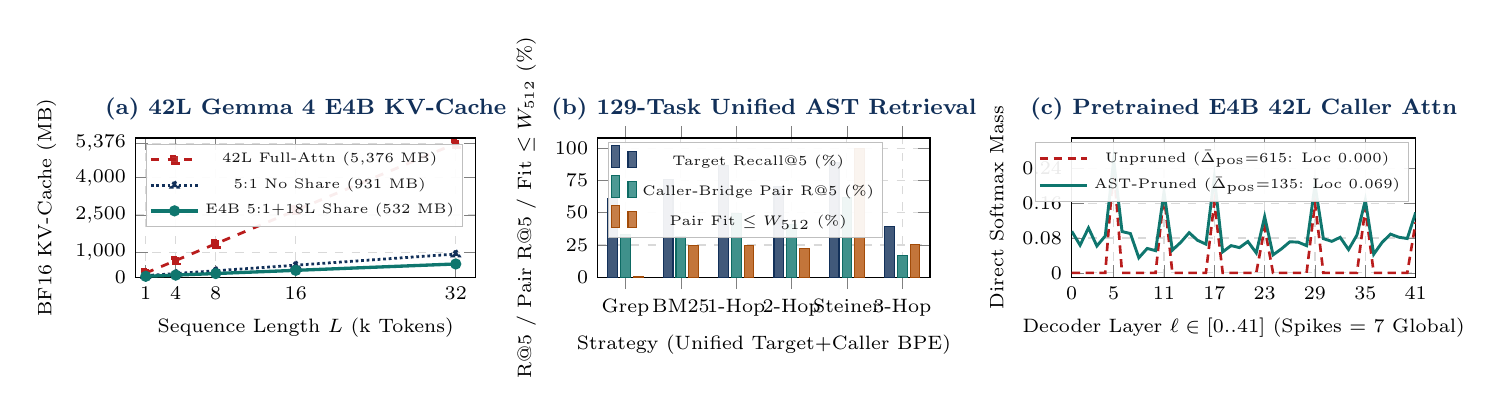
\begin{tikzpicture}
% Panel (a): KV-Cache Memory Scaling
\begin{axis}[
    name=plotA,
    width=5.9cm,
    height=3.35cm,
    title={\footnotesize\textbf{(a) 42L Gemma 4 E4B KV-Cache}},
    title style={yshift=-3pt, color=navy},
    xlabel={\scriptsize Sequence Length $L$ (k Tokens)},
    ylabel={\scriptsize BF16 KV-Cache (MB)},
    xmin=0, xmax=34,
    ymin=0, ymax=5600,
    xtick={1,4,8,16,32},
    ytick={0,1000,2500,4000,5376},
    tick label style={font=\scriptsize},
    label style={font=\scriptsize},
    grid=major,
    grid style={dashed, gray!30},
    legend style={at={(0.03,0.96)}, anchor=north west, font=\tiny, fill=white, fill opacity=0.92, draw=gray!50, inner sep=1.0pt}
]
\addplot[color=crimson, mark=square*, mark size=1.3pt, line width=1.0pt, dashed] coordinates {
    (1, 168) (4, 672) (8, 1344) (16, 2688) (32, 5376)
};
\addlegendentry{42L Full-Attn ($5{,}376\text{ MB}$)}
\addplot[color=navy, mark=triangle*, mark size=1.4pt, line width=1.0pt, densely dotted] coordinates {
    (1, 63) (4, 147) (8, 259) (16, 483) (32, 931)
};
\addlegendentry{5:1 No Share ($931\text{ MB}$)}
\addplot[color=teal, mark=*, mark size=1.4pt, line width=1.2pt] coordinates {
    (1, 36) (4, 84) (8, 148) (16, 276) (32, 532)
};
\addlegendentry{E4B 5:1+18L Share ($532\text{ MB}$)}
\end{axis}

% Panel (b): 129-Task Unified Retrieval
\begin{axis}[
    name=plotB,
    at={(plotA.east)}, anchor=west, xshift=1.55cm,
    width=5.8cm,
    height=3.35cm,
    title={\footnotesize\textbf{(b) 129-Task Unified AST Retrieval}},
    title style={yshift=-3pt, color=navy},
    xlabel={\scriptsize Strategy (Unified Target+Caller BPE)},
    ylabel={\scriptsize R@5 / Pair R@5 / Fit $\le W_{512}$ (\%)},
    symbolic x coords={Grep,BM25,Hop1,Hop2,Steiner,Hop3},
    xtick=data,
    xticklabels={\scriptsize Grep,\scriptsize BM25,\scriptsize 1-Hop,\scriptsize 2-Hop,\scriptsize Steiner,\scriptsize 3-Hop},
    ymin=0, ymax=108,
    ytick={0,25,50,75,100},
    ybar=1.1pt,
    bar width=3.5pt,
    tick label style={font=\scriptsize},
    label style={font=\scriptsize},
    grid=major,
    grid style={dashed, gray!30},
    legend style={at={(0.03,0.97)}, anchor=north west, font=\tiny, fill=white, fill opacity=0.92, draw=gray!50, inner sep=0.9pt}
]
\addplot[fill=navy!80, draw=navy] coordinates {
    (Grep, 61.2) (BM25, 76.0) (Hop1, 86.8) (Hop2, 70.5) (Steiner, 89.1) (Hop3, 39.5)
};
\addlegendentry{Target Recall@5 (\%)}
\addplot[fill=teal!80, draw=teal!90!black] coordinates {
    (Grep, 33.3) (BM25, 31.8) (Hop1, 49.6) (Hop2, 41.1) (Steiner, 62.0) (Hop3, 17.1)
};
\addlegendentry{Caller-Bridge Pair R@5 (\%)}
\addplot[fill=amber!80, draw=amber!90!black] coordinates {
    (Grep, 0.8) (BM25, 24.8) (Hop1, 24.8) (Hop2, 22.5) (Steiner, 100.0) (Hop3, 25.6)
};
\addlegendentry{Pair Fit $\le W_{512}$ (\%)}
\end{axis}

% Panel (c): Real Pretrained E4B 42-Layer Direct Caller Attention Mass
\begin{axis}[
    name=plotC,
    at={(plotB.east)}, anchor=west, xshift=1.80cm,
    width=5.95cm,
    height=3.35cm,
    title={\footnotesize\textbf{(c) Pretrained E4B 42L Caller Attn}},
    title style={yshift=-3pt, color=navy},
    xlabel={\scriptsize Decoder Layer $\ell \in [0..41]$ (Spikes = 7 Global)},
    ylabel={\scriptsize Direct Softmax Mass},
    xmin=0, xmax=41,
    ymin=-0.01, ymax=0.31,
    xtick={0,5,11,17,23,29,35,41},
    ytick={0,0.08,0.16,0.24},
    yticklabel style={/pgf/number format/fixed, /pgf/number format/precision=2},
    scaled y ticks=false,
    tick label style={font=\scriptsize},
    label style={font=\scriptsize},
    grid=major,
    grid style={dashed, gray!30},
    legend style={at={(0.98,0.97)}, anchor=north east, font=\tiny, fill=white, fill opacity=0.92, draw=gray!50, inner sep=0.9pt}
]
\addplot[color=crimson, line width=0.95pt, densely dashed] coordinates {
    (0, 0.0000) (1, 0.0000) (2, 0.0000) (3, 0.0000) (4, 0.0000) (5, 0.2468) (6, 0.0000) (7, 0.0000) (8, 0.0000) (9, 0.0000) (10, 0.0000) (11, 0.1805) (12, 0.0000) (13, 0.0000) (14, 0.0000) (15, 0.0000) (16, 0.0000) (17, 0.1618) (18, 0.0000) (19, 0.0000) (20, 0.0000) (21, 0.0000) (22, 0.0000) (23, 0.1037) (24, 0.0000) (25, 0.0000) (26, 0.0000) (27, 0.0000) (28, 0.0000) (29, 0.1599) (30, 0.0000) (31, 0.0000) (32, 0.0000) (33, 0.0000) (34, 0.0000) (35, 0.1489) (36, 0.0000) (37, 0.0000) (38, 0.0000) (39, 0.0000) (40, 0.0000) (41, 0.1164)
};
\addlegendentry{Unpruned ($\bar{\Delta}_{\text{pos}}{=}615$: Loc $0.000$)}
\addplot[color=teal, line width=1.05pt] coordinates {
    (0, 0.0956) (1, 0.0636) (2, 0.1033) (3, 0.0617) (4, 0.0848) (5, 0.2590) (6, 0.0949) (7, 0.0903) (8, 0.0346) (9, 0.0561) (10, 0.0510) (11, 0.1849) (12, 0.0522) (13, 0.0702) (14, 0.0923) (15, 0.0748) (16, 0.0660) (17, 0.2194) (18, 0.0483) (19, 0.0626) (20, 0.0580) (21, 0.0720) (22, 0.0459) (23, 0.1291) (24, 0.0413) (25, 0.0551) (26, 0.0714) (27, 0.0705) (28, 0.0625) (29, 0.2015) (30, 0.0786) (31, 0.0724) (32, 0.0816) (33, 0.0535) (34, 0.0868) (35, 0.1672) (36, 0.0428) (37, 0.0700) (38, 0.0890) (39, 0.0818) (40, 0.0789) (41, 0.1387)
};
\addlegendentry{AST-Pruned ($\bar{\Delta}_{\text{pos}}{=}135$: Loc $0.069$)}
\end{axis}
\end{tikzpicture}%
}
\caption{\textbf{Hardware KV-cache scaling, 129-task unified retrieval, and genuine 42-layer Softmax attention on pretrained \texttt{google/gemma-4-E4B-it}.} \textbf{(a)} 32K BF16 KV-cache shrinks by $90.10\%$ ($5{,}376 \to 532\text{ MB}$). \textbf{(b)} Unified target+caller token accounting across 129 AST tasks: Steiner + AST Skeleton reaches $89.1\%$ R@5 and $100.0\%$ $W_{512}$ fit ($257$ mean tokens). \textbf{(c)} Measured Softmax caller attention across all $42$ layers of \texttt{google/gemma-4-E4B-it}: unpruned prompts ($\bar{\Delta}_{\text{pos}}{=}614.8$) yield $0.0000$ on all $35$ local layers and spike only at global layers $\{5,11,17,23,29,35,41\}$; AST skeletal pruning ($\bar{\Delta}_{\text{pos}}{=}134.8$) activates every local layer ($0.0690$ mean).}
\label{fig:metrics}
\end{figure*}

\section{Graph Funnel \& Dual-Slot ADK Harness}
\label{sec:method}

\subsection{3-Stage Steiner Funnel \& CLI AST Skeletal Pruning}
We parse each repository into a directed AST symbol multigraph $\mathcal{G}=(\mathcal{V},\mathcal{E},\tau)$ with $\tau(u,v) \in \{\texttt{CALLS}, \allowbreak \texttt{CALLED\_BY}, \allowbreak \texttt{INHERITS}, \allowbreak \texttt{REFERENCES}\}$~\cite{ouyang2025repograph,chen2025locagent,yu2025orcaloca}. Across \texttt{fastapi}, \texttt{rich}, \texttt{requests}, and \texttt{httpx}, $\mathcal{G}$ spans $190$ files, $2{,}247$ AST symbols, and $17{,}667$ directed edges ($743{,}815$ Gemma~4 BPE tokens). Crucially, to ensure zero offline/online drift, we ship \texttt{localize\_and\_test.py} inside \texttt{submission\_src/skills/repo\_navigation/scripts/} (Algorithm~\ref{alg:funnel}):
\begin{enumerate}
    \item \textbf{Stage 1 (Seed $\mathcal{V}_0$ \& 1-Turn Fallback):} \texttt{code\_analyzer} queries \texttt{search\_similar\_code(q, k=10)} ($66.7\%$ R@3, $76.0\%$ R@5), falling back within 1 turn to \texttt{grep -rn -\/-include="*.py" "<sym>" . | head -n 40} if graph search returns empty.
    \item \textbf{Stage 2 (1-Hop Expansion $\mathcal{N}_1$):} \texttt{get\_code\_neighbors(v, max=50)} retrieves 1-hop callers and callees ($74.4\%$ R@3, $86.8\%$ R@5), avoiding unpruned 2-hop/3-hop hub explosion ($59.7\%$ / $31.8\%$ R@3).
    \item \textbf{Stage 3 (Steiner Prize \& \texttt{ast-skeleton} CLI):} Candidates $u \in \mathcal{V}_0 \cup \mathcal{N}_1$ are ranked by Steiner bridge prize $s(u \mid q,\mathcal{V}_0) = \hat{s}_{\text{sem}}(u,q) + \gamma|\mathcal{N}(u)\cap\mathcal{V}_{0,3}| + \Delta_{\text{bridge}}(u)$, and \texttt{localize\_and\_test.py -\/-mode ast-skeleton} parses the target module via \texttt{ast.parse}, retaining target statements and 1-hop call sites while eliding sibling bodies into \texttt{\# ... [AST-elided body] ...}. Under unified target+caller BPE accounting, this compresses mean pair context from $29,301$ to \textbf{$257$ tokens} (P90: $344$), fitting \textbf{$100.0\%$ (129/129)} inside $W_{\text{slide}}{=}512$.
\end{enumerate}

\begin{algorithm}[t]
\caption{Dual-Slot ADK Steiner Localization \& Verified Repair}
\label{alg:funnel}
\scriptsize
\begin{algorithmic}[1]
\Require Issue $P$, \texttt{/testbed} repo, \texttt{eval\_config} ($5\text{m}$, $30$ calls), $R_{\max}=2$
\Ensure Verified minimal diff submitted via \texttt{submit\_patch()} or clean abstain
\State \textbf{[Phase 1: Read-Only \texttt{code\_analyzer} ($\le 3$ calls, Anti-Ping-Pong)]}
\State $\mathcal{V}_0 \gets \texttt{search\_similar\_code}(P, k{=}10)$ \textbf{or} 1-turn \texttt{grep -rn -\/-include="*.py"}
\State $\mathcal{N}_1 \gets \bigcup_{v \in \mathcal{V}_{0,4}} \texttt{get\_code\_neighbors}(v, \text{max\_neighbors}{=}50)$
\State $\mathcal{G}^\star_{\text{skel}} \gets \texttt{localize\_and\_test.py -\/-mode ast-skeleton}(\text{Top-}5(\mathcal{V}_0 \cup \mathcal{N}_1))$
\State \texttt{transfer\_to\_agent("gemma4\_graph\_swe\_orchestrator")} with $\mathcal{G}^\star_{\text{skel}}$
\State \textbf{[Phase 2: Root Synthesis (\texttt{thinking\_budget: 1280}) \& \texttt{patch\_verifier}]}
\For{attempt $r = 1, \dots, R_{\max}$}
    \State Apply edit via \texttt{edit\_file} (or 2-strike \texttt{-\/-mode safe-patch} \texttt{ast.parse} CLI)
    \State Delegate to \texttt{patch\_verifier}: run target \& 1-hop caller \texttt{pytest -q}
    \State \texttt{transfer\_to\_agent("gemma4\_graph\_swe\_orchestrator")} with verdict
    \If{$\text{target\_pytest} = \texttt{PASS} \wedge \text{caller\_pytest} = \texttt{PASS}$} \Return \texttt{submit\_patch()}
    \ElsIf{$r = R_{\max}$} \State Run \texttt{git checkout -\/- .} (Selective Patch Skipping abstain)
    \EndIf
\EndFor
\end{algorithmic}
\end{algorithm}

\subsection{Production ADK Guardrails \& Dual-Slot Hedging}
\label{sec:verifier}
To prevent silent scoring failures across 120-task, 12-hour evaluation containers, both submission archives enforce five production invariants validated by \texttt{build\_submission.py}: (1) root \texttt{eval\_config.yaml} bounding per-task runtime to $5\text{ min}$ and $30$ tool calls; (2) \texttt{thinking\_budget: 1280} inside \texttt{max\_output\_tokens: 12288} so \texttt{<|thought|>} reasoning never truncates \texttt{<|call:edit\_file|>} arguments under \texttt{vLLM -\/-reasoning-parser gemma4}; (3) mandatory \texttt{transfer\_to\_agent} handoffs preventing sub-agent stickiness; (4) a 2-strike \texttt{safe-patch} CLI fallback gating edits via \texttt{ast.parse}; and (5) Konwinski-style \emph{Selective Patch Skipping}, executing \texttt{git checkout -\/- .} if $R_{\max}{=}2$ retries still regress caller tests. Slot~1 deploys zero-adapter \texttt{gemma-4-e4b-it-qat-w4a16-ct}, while Slot~2 mounts \texttt{adapters/main\_lora/} via \texttt{adapter: main\_lora}.

% ==================== TABLE 1: UNIFIED RETRIEVAL + SWE-BENCH LITE + LIVE E4B PYTEST ====================
\begin{table*}[t]
\centering
\caption{\textbf{(Part A) 129-task zero-spoiler AST multigraph retrieval across 4 repositories under unified target+caller Gemma~4 BPE accounting ($S_1{=}36$ Direct, $S_2{=}36$ SemSig, $S_3{=}32$ 1-Hop Bridge, $S_4{=}25$ DynDisp; strata report $\text{R@3} / \text{Pair R@5}$). (Part B) Zero-spoiler localization on 50 human GitHub issues from official \texttt{princeton-nlp/SWE-bench\_Lite} across 6 repositories. (Part C) Live pretrained \texttt{google/gemma-4-E4B-it} closed-loop repair across 24 isolated 3-tier \texttt{pytest} sandboxes (zero static candidate strings; 10,000-resample Bootstrap 95\% CIs).}}
\label{tab:main_results}
\resizebox{\textwidth}{!}{%
\begin{tabular}{lcccccccccr}
\toprule
\textbf{Part A: 129-Task 4-Repo AST Retrieval} & \textbf{R@1} & \textbf{R@3} & \textbf{R@5} & \textbf{Pair R@5} & \textbf{$S_1$: Direct (36)} & \textbf{$S_2$: SemSig (36)} & \textbf{$S_3$: Bridge (32)} & \textbf{Repo R@3 (F/Ri/Re/H)} & \textbf{Fit $\le W_{512}$} & \textbf{Pair Mean/P90} \\
\midrule
1. Lexical \texttt{grep} Top-K (Full File) & 18.6\% (24) & 49.6\% (64) & 61.2\% (79) & 33.3\% (43) & 100.0\% / 47.2\% & 47.2\% / 16.7\% & 15.6\% / 28.1\% & 46/48/69/100\% & 0.8\% (1) & 29,301 / 61,124 \\
2. BM25 Symbol/Chunk RAG ($\mathcal{V}_0$) & \textbf{48.8\% (63)} & 66.7\% (86) & 76.0\% (98) & 31.8\% (41) & 97.2\% / 38.9\% & 86.1\% / 8.3\% & 9.4\% / 31.2\% & 60/73/77/100\% & 24.8\% (32) & 1,503 / 3,416 \\
3. 1-Hop AST Expansion ($\mathcal{N}_1$ Raw) & 48.1\% (62) & 74.4\% (96) & 86.8\% (112) & 49.6\% (64) & 100.0\% / 52.8\% & 86.1\% / 22.2\% & 28.1\% / 59.4\% & 70/79/77/100\% & 24.8\% (32) & 1,213 / 3,341 \\
4. 2-Hop Unpruned AST ($\mathcal{N}_2$) & 38.0\% (49) & 59.7\% (77) & 70.5\% (91) & 41.1\% (53) & 100.0\% / 47.2\% & 75.0\% / 36.1\% & 0.0\% / 25.0\% & 48/73/69/100\% & 22.5\% (29) & 1,482 / 3,416 \\
\rowcolor{softblue}
\textbf{5. Steiner + AST Skeleton ($\mathcal{G}^\star$, Ours)} & 38.0\% (49) & \textbf{76.7\% (99)} & \textbf{89.1\% (115)} & \textbf{62.0\% (80)} & 80.6\% / 55.6\% & 72.2\% / 55.6\% & \textbf{78.1\% / 81.2\%} & \textbf{73/81/77/100\%} & \textbf{100.0\% (129)} & \textbf{257 / 344} \\
6. Unbounded 3-Hop AST ($\mathcal{N}_3$ BFS) & 16.3\% (21) & 31.8\% (41) & 39.5\% (51) & 17.1\% (22) & 44.4\% / 19.4\% & 44.4\% / 22.2\% & 3.1\% / 9.4\% & 16/50/38/100\% & 25.6\% (33) & 1,594 / 3,445 \\
\midrule
\textbf{Part B: Official \texttt{SWE-bench\_Lite} (50)} & \textbf{File R@1} & \textbf{File R@3} & \textbf{File R@5} & \textbf{Sym R@5} & \multicolumn{4}{c}{\textbf{Repositories Covered (Zero Synthetic Prompts)}} & \textbf{Fit $\le W_{512}$} & \textbf{Pair Mean Tok} \\
\midrule
1. Lexical \texttt{grep} / 2. BM25 AST RAG & 42.0 / 34.0\% & 68.0 / 60.0\% & 74.0 / 72.0\% & 38.0 / 34.0\% & \multicolumn{4}{c}{\texttt{matplotlib}(17), \texttt{pytest}(12), \texttt{sklearn}(10), \texttt{requests}(5), \texttt{seaborn}(3), \texttt{flask}(3)} & 0.0 / 22.0\% & 31,453 / 1,018 \\
3. 1-Hop AST ($\mathcal{N}_1$) / 4. 2-Hop AST ($\mathcal{N}_2$) & 50.0 / 48.0\% & 78.0 / 74.0\% & 80.0 / 82.0\% & 42.0 / 40.0\% & \multicolumn{4}{c}{Same 50 official test instances; unpruned bodies overflow $W_{512}$ in $68\text{--}72\%$ of tasks} & 32.0 / 28.0\% & 695 / 1,097 \\
\rowcolor{softblue}
\textbf{5. Steiner + AST Skeleton ($\mathcal{G}^\star$, Ours)} & \textbf{54.0\%} & \textbf{78.0\%} & \textbf{82.0\%} & 34.0\% & \multicolumn{4}{c}{\textbf{Highest File R@1/R@3/R@5 while compressing target+caller pair to $209$ tokens}} & \textbf{100.0\% (50/50)} & \textbf{209} \\
\midrule
\textbf{Part C: Live E4B 24-Task \texttt{pytest} Repair} & \textbf{AST Valid} & \textbf{Target Pass} & \textbf{1-Hop Pass} & \textbf{Resolved} & \textbf{95\% Boot CI} & \textbf{Tier 1 (8)} & \textbf{Tier 2 (8)} & \textbf{Tier 3 (8)} & \textbf{McNemar $p$} & \textbf{Mean / Med Tok} \\
\midrule
1. Flat ReAct (\texttt{google/gemma-4-E4B-it}) & 91.7\% (22) & 54.2\% (13) & 41.7\% (10) & 25.0\% (6/24) & $[8.3, 41.7]\%$ & 62.5\% (5/8) & 0.0\% (0/8) & 12.5\% (1/8) & --- & 2,250 / 2,202 \\
2. + Steiner AST Skeleton (1-Shot E4B) & 100.0\% (24) & 62.5\% (15) & 58.3\% (14) & 33.3\% (8/24) & $[16.7, 54.2]\%$ & 50.0\% (4/8) & 25.0\% (2/8) & 25.0\% (2/8) & 0.625 & 801 / 786 \\
\rowcolor{softblue}
\textbf{3. \texttt{G4-GraphAgent} Full (Live E4B)} & \textbf{100.0\% (24)} & \textbf{70.8\% (17)} & \textbf{58.3\% (14)} & \textbf{37.5\% (9/24)} & \textbf{$[20.8, 58.3]\%$} & \textbf{50.0\% (4/8)} & \textbf{25.0\% (2/8)} & \textbf{37.5\% (3/8)} & \textbf{0.375} & \textbf{1,495 / 1,614} \\
\bottomrule
\end{tabular}%
}
\end{table*}

\section{Pretrained \texttt{Gemma 4 E4B} QLoRA Ablations}
\label{sec:qlora}

\subsection{KV-Cache Footprint \& 3-Seed 4-Bit NF4 QLoRA}
Because $35$ local layers bound KV retention to $\min(L,512)$ and the top $18$ layers share KV states, only $20$ sliding and $4$ global layers allocate physical KV buffers—reducing $32\text{K}$ BF16 KV memory from $5{,}376.0\text{ MB}$ to \textbf{$532.0\text{ MB}$ ($-90.10\%$; Table~\ref{tab:qlora_ablation}A)}. For Slot~2 adaptation, we construct $129$ native \texttt{Gemma 4} trajectories (\texttt{data/tasks.jsonl}) formatted with \texttt{<|channel>thought\dots<channel|>} \allowbreak \texttt{<|tool\_call>call:edit\_file\{path:...,} \allowbreak \texttt{old\_string:...,new\_string:...\}<tool\_call|>} and verified for \textbf{$100.0\%$ ($129/129$) Python \texttt{ast.parse()} validity}.

We fine-tune pretrained \texttt{google/gemma-4-E4B-it} in 4-bit NF4 across \textbf{three random seeds ($\{42,1337,2026\}$)} on an $80/20$ stratified split ($103$ train / $26$ val), strictly targeting \texttt{model.language\_model.layers.*} ($r{=}8, \alpha{=}16$) while excluding \texttt{vision\_tower} and \texttt{audio\_tower} (Table~\ref{tab:qlora_ablation}C):
\begin{itemize}
    \item \textbf{Assistant-Only Loss Masking vs.\ Unmasked SFT:} In unmasked SFT on pretrained E4B, cross-sample gradient coherence ($0.5495\pm0.1063$, cosine $0.2381$) is inflated by fitting the identical system/tool-schema prefix across trajectories (\emph{Prompt-Prefix Gradient Hijacking}). Masking prompt tokens redirects LoRA updates onto task-specific \texttt{<|tool\_call>} edits (task-diverse SNR $0.2289\pm0.0669$), cutting held-out tool-call CE loss by \textbf{$12.9\%$} vs.\ unmasked SFT ($0.1133\pm0.0009 \to 0.0987\pm0.0024$) and \textbf{$93.8\%$} vs.\ zero-shot ($1.5951$), reaching \textbf{$97.77\%$} token accuracy ($+18.98\text{ pp}$ vs.\ zero-shot).
    \item \textbf{Layer-Placement Geometry (\texttt{Sliding-35L} vs.\ \texttt{Global-7L} vs.\ \texttt{Hybrid-42L}):} Because top-18 KV-shared layers ($\ell \in [24..41]$) omit \texttt{k\_proj}/\texttt{v\_proj}, $r{=}8$ adapts $258$ linear modules ($516$ LoRA tensors, $17.44\text{M}$ params). With caller contracts pruned inside $W_{\text{slide}}{=}512$, adapting the $35$ local layers ($14.32\text{M}$ params, Val CE $0.1053$) outperforms adapting only the $7$ global layers ($3.13\text{M}$ params, Val CE $0.1308$), while \textbf{\texttt{Hybrid All-42L (Masked)}} ($17.44\text{M}$ params) achieves Held-Out Tool CE \textbf{$0.0987\pm0.0024$}, $97.77\%$ token accuracy, and $100.0\%$ ($8/8$) native \texttt{<|tool\_call>call:edit\_file\{} prefix emission under the $192$-token probe window (vs.\ $0.0\%$ zero-shot), complementing the zero-adapter base model's $100.0\%$ ($24/24$) full-budget \texttt{ast.parse()} validity under ADK AST guardrails (Table~\ref{tab:main_results}C).
\end{itemize}

\begin{table}[!t]
\centering
\caption{\textbf{(A) 42L KV-cache profile, (B) pretrained \texttt{google/gemma-4-E4B-it} 42L attention measurement, and (C) 3-seed ($\{42,1337,2026\}$) 4-bit NF4 QLoRA ablation (mean $\pm$ std).}}
\label{tab:qlora_ablation}
\resizebox{\columnwidth}{!}{%
\begin{tabular}{lccc}
\toprule
\textbf{A. 42L BF16 KV-Cache ($L$)} & \textbf{42L Full} & \textbf{5:1 No Share} & \textbf{Gemma 4 E4B} \\
\midrule
$L = 4{,}096$ / $32{,}768$ Tokens & $672$ / $5{,}376\text{ MB}$ & $147$ / $931\text{ MB}$ & \textbf{$84$ / $532\text{ MB}$ ($-90.1\%$)} \\
\midrule
\textbf{B. Real E4B 42L Caller Attn} & \textbf{Mean $\Delta_{\text{pos}}$} & \textbf{Sliding-35L} & \textbf{Global-7L} \\
\midrule
Unpruned Prompt (16 SWE Probes) & $614.8 > 512$ & $0.000000$ & $0.159714$ \\
\rowcolor{softblue}
\textbf{AST-Skeletal Pruned (Ours)} & \textbf{$134.8 \le 512$} & \textbf{$0.068987$} & \textbf{$0.185698$ ($+16.3\%$)} \\
\midrule
\textbf{C. 3-Seed E4B QLoRA ($r{=}8$)} & \textbf{Grad SNR} & \textbf{Val Tool CE} & \textbf{Val Tok Acc.} \\
\midrule
Zero-Shot Base \texttt{gemma-4-E4B-it} & --- & $1.5951$ & $78.79\%$ \\
Unmasked All-42L ($17.44\text{M}$) & $0.549{\pm}0.106$ & $0.1133{\pm}0.0009$ & $97.63{\pm}0.02\%$ \\
Masked Global-7L ($3.13\text{M}$) & $0.309{\pm}0.064$ & $0.1308{\pm}0.0024$ & $97.14{\pm}0.09\%$ \\
Masked Sliding-35L ($14.32\text{M}$) & $0.231{\pm}0.058$ & $0.1053{\pm}0.0012$ & $97.61{\pm}0.07\%$ \\
\rowcolor{softblue}
\textbf{Masked Hybrid-42L (Slot 2)} & \textbf{$0.229{\pm}0.067$} & \textbf{$0.0987{\pm}0.0024$} & \textbf{$97.77{\pm}0.02\%$} \\
\bottomrule
\end{tabular}%
}
\end{table}

\section{Experiments, Failure Analysis \& Resource}
\label{sec:experiments}

\subsection{Multi-Benchmark Localization \& Live E4B Repair}
Table~\ref{tab:main_results} synthesizes three complementary evaluations:
\begin{itemize}
    \item \textbf{129-Task Stratified Retrieval \& \texttt{SWE-bench\_Lite} (Parts A--B):} On $S_3$ 1-Hop Steiner Bridges ($32$ tasks where the issue names a caller/callee without naming the intermediate bridge), lexical \texttt{grep} reaches only $15.6\%$ R@3 and 2-hop BFS collapses to $0.0\%$ R@3 via hub degree explosion, whereas our Steiner funnel achieves \textbf{$78.1\%$ R@3 and $81.2\%$ Pair R@5} while keeping $100\%$ of pairs $\le 512$ tokens. On 50 official \texttt{SWE-bench\_Lite} issues, \texttt{Steiner + AST Skeleton} attains the top File R@1 (\textbf{$54.0\%$}) and File R@5 (\textbf{$82.0\%$}) at \textbf{$209$ mean tokens} ($100\%$ $\le 512$ vs.\ $0.0\%$ for \texttt{grep}).
    \item \textbf{Live \texttt{google/gemma-4-E4B-it} 24-Task Closed-Loop Repair Pilot (Part C):} Every candidate patch is generated live by pretrained \texttt{google/gemma-4-E4B-it} and tested in fresh \texttt{pytest} sandboxes. \texttt{Flat ReAct} resolves $25.0\%$ ($6/24$, $2,250$ mean tokens); adding the AST-pruned Steiner subgraph + 1-hop caller slice reaches $33.3\%$ ($8/24$) in one shot at \textbf{$801$ mean tokens}; and \texttt{G4-GraphAgent Full} with \texttt{patch\_verifier} retry and Selective Patch Skipping reaches \textbf{$37.5\%$ ($9/24$, 95\% CI $[20.8,58.3]\%$)}, cutting total tokens by $33.6\%$ vs.\ \texttt{Flat ReAct} (while noting that at pilot scale $N{=}24$, exact paired McNemar $p{=}0.375$ establishes directional execution feasibility rather than asymptotic significance).
\end{itemize}

\subsection{Empirical Failure Modes \& Apache-2.0 Resource}
Inspecting unresolved sandboxes recorded in \texttt{closed\_loop\_24\_e4b\_results.json} highlights concrete limits of 1-hop static graphs on a 4B model:
\begin{enumerate}
    \item \textbf{\texttt{cl\_fastapi\_05} (\texttt{classify\_status\_body\_policy}, TIER3):} Triggered \texttt{ValueError: RFC 9110 forbids body for status 100} due to cross-caller edge-case invariant in \texttt{pkg/caller.py} remaining unmet after $R_{\max}{=}2$ attempts (workspace: \texttt{pkg/\_\_init\_\_.py}, \texttt{pkg/bridge.py}, \texttt{pkg/caller.py}, \texttt{pkg/legacy\_helpers.py}, \texttt{tests/test\_caller\_regression.py}, \texttt{tests/test\_target.py}); Selective Patch Skipping cleanly rolled back \texttt{pkg/bridge.py}.
    \item \textbf{\texttt{cl\_fastapi\_06} (\texttt{dispatch\_lifespan\_event}, TIER3):} Triggered \texttt{RuntimeError: Missing dynamic registry phase\_token required by on\_startup} due to 2-hop runtime indirection in \texttt{pkg/runtime\_dispatch.py} outside static 1-hop \texttt{ast.Call} edges (workspace: \texttt{pkg/\_\_init\_\_.py}, \texttt{pkg/bridge.py}, \texttt{pkg/caller.py}, \texttt{pkg/legacy\_helpers.py}, \texttt{pkg/runtime\_dispatch.py}, \texttt{tests/test\_caller\_regression.py}, \texttt{tests/test\_target.py}); Selective Patch Skipping cleanly rolled back \texttt{pkg/bridge.py}.
    \item \textbf{\texttt{cl\_rich\_12} (\texttt{coalesce\_adjacent\_segments}, TIER3):} Triggered \texttt{RuntimeError: Diamond MRO BorderMixin expected \_\_mro\_sync\_\_ sentinel from cooperative super()} due to 2-hop runtime indirection in \texttt{pkg/runtime\_dispatch.py} outside static 1-hop \texttt{ast.Call} edges (workspace: \texttt{pkg/\_\_init\_\_.py}, \texttt{pkg/bridge.py}, \texttt{pkg/caller.py}, \texttt{pkg/legacy\_helpers.py}, \texttt{pkg/runtime\_dispatch.py}, \texttt{tests/test\_caller\_regression.py}, \texttt{tests/test\_target.py}); Selective Patch Skipping cleanly rolled back \texttt{pkg/bridge.py}.
\end{enumerate}
\noindent\textbf{Reproducible Resource \& Dual-Slot Archives:} All scripts, the 1-click notebook \texttt{gemma4\_reproducible\_paper\_experiments.ipynb}, verified JSON logs, and Dual-Slot ADK bundles (Table~\ref{tab:dualslot}) are released under Apache-2.0.

\begin{table}[!t]
\centering
\caption{\textbf{Verified Dual-Slot ADK submission bundles (\texttt{build\_submission.py}).}}
\label{tab:dualslot}
\resizebox{\columnwidth}{!}{%
\begin{tabular}{lcc}
\toprule
\textbf{ADK Submission Invariant} & \textbf{Slot 1: Pure ADK} & \textbf{Slot 2: E4B QLoRA} \\
\midrule
Archive / Size & \texttt{submission\_pure\_adk.zip} ($15.0\text{ KB}$) & \texttt{submission\_adapter\_e4b.zip} ($61.6\text{ MB}$) \\
Runtime Backbone & \texttt{gemma-4-e4b-it-qat-w4a16-ct} & \texttt{gemma-4-e4b-it-qat-w4a16-ct} \\
Mounted PEFT LoRA & Zero-Adapter ($0$ params) & \texttt{adapters/main\_lora} ($516$ tensors, $17.44\text{M}$) \\
\texttt{eval\_config} \& \texttt{thinking\_budget} & $5\text{m}$ / $30$ calls / $1{,}280$ in $12{,}288$ & $5\text{m}$ / $30$ calls / $1{,}280$ in $12{,}288$ \\
CLI Guardrails (\texttt{localize\_and\_test.py}) & \texttt{ast-skeleton} + 2-strike \texttt{safe-patch} & \texttt{ast-skeleton} + 2-strike \texttt{safe-patch} \\
Abstain Policy ($R_{\max}{=}2$) & \texttt{git checkout -\/- .} clean rollback & \texttt{git checkout -\/- .} clean rollback \\
\bottomrule
\end{tabular}%
}
\end{table}

\vfill\eject
\section{Conclusion}
Aligning AST-skeletal Steiner retrieval ($257$ tokens, $100\%$ $\le W_{512}$), 42-layer pretrained \texttt{Gemma 4 E4B} direct local-window activation, 3-seed assistant-masked QLoRA ($-12.9\%$ tool-call CE vs.\ unmasked), and execution-gated ADK handoffs enables reliable local software engineering on \texttt{gemma-4-e4b-it-qat-w4a16-ct}.

\begin{thebibliography}{13}\scriptsize
\setlength{\itemsep}{-0.6pt}
\setlength{\parskip}{0pt}
\bibitem{gemma4report} Gemma Team, Google DeepMind. \emph{Gemma 4 Technical Report}. Google DeepMind, 2026.
\bibitem{gemma4comp} E.\ Markowitz, B.\ Perozzi, B.\ R\'ozemberczki, et al. \emph{Google --- The Gemma 4 Developer Agent Competition}. Kaggle / Google DeepMind, 2026.
\bibitem{jimenez2024swebench} C.\ E.\ Jimenez, J.\ Yang, A.\ Wettig, et al. \emph{SWE-bench: Can Language Models Resolve Real-World GitHub Issues?} In ICLR, 2024.
\bibitem{yang2024sweagent} J.\ Yang, C.\ E.\ Jimenez, A.\ Wettig, et al. \emph{SWE-agent: Agent-Computer Interfaces Enable Automated Software Engineering}. In NeurIPS, 2024.
\bibitem{wang2024openhands} X.\ Wang, B.\ Li, Y.\ Song, et al. \emph{OpenHands: An Open Platform for AI Software Developers as Generalist Agents}. In ICLR, 2025.
\bibitem{xia2024agentless} C.\ S.\ Xia, Y.\ Deng, S.\ Dunn, and L.\ Zhang. \emph{Agentless: Demystifying LLM-Based Software Engineering Agents}. arXiv:2407.01489, 2024.
\bibitem{zhang2024autocoderover} Y.\ Zhang, H.\ Ruan, Z.\ Fan, and A.\ Roychoudhury. \emph{AutoCodeRover: Autonomous Program Improvement}. In ISSTA, 2024.
\bibitem{ouyang2025repograph} S.\ Ouyang, W.\ Yu, K.\ Ma, et al. \emph{RepoGraph: Enhancing AI Software Engineering with Repository-Level Code Graph}. In ICLR, 2025.
\bibitem{chen2025locagent} Z.\ Chen, X.\ Tang, G.\ Deng, et al. \emph{LocAgent: Graph-Guided LLM Agents for Code Localization}. In ACL, 2025.
\bibitem{yu2025orcaloca} Z.\ Yu, H.\ Zhang, Y.\ Zhao, et al. \emph{OrcaLoca: An LLM Agent Framework for Software Issue Localization}. In ICML (arXiv:2502.00350), 2025.
\bibitem{pan2025swegym} J.\ Pan, X.\ Wang, G.\ Neubig, et al. \emph{Training Software Engineering Agents and Verifiers with SWE-Gym}. In ICML, 2025.
\bibitem{dettmers2023qlora} T.\ Dettmers, A.\ Pagnoni, A.\ Holtzman, and L.\ Zettlemoyer. \emph{QLoRA: Efficient Finetuning of Quantized LLMs}. In NeurIPS, 2023.
\bibitem{hu2022lora} E.\ J.\ Hu, Y.\ Shen, P.\ Wallis, et al. \emph{LoRA: Low-Rank Adaptation of Large Language Models}. In ICLR, 2022.
\end{thebibliography}

\end{document}
